\documentclass[a4paper,12pt]{article}

% Paquetes básicos
\usepackage[utf8]{inputenc}
\usepackage[T1]{fontenc}
\usepackage[spanish]{babel}
\usepackage{graphicx}
\usepackage{xcolor}
\usepackage{lipsum}
\usepackage{geometry}
\geometry{top=3cm, bottom=3cm, left=2.5cm, right=2.5cm}



% Paquetes para diseño
\usepackage{titlesec}
\usepackage{fancyhdr}
\usepackage{amsmath}
\usepackage{amssymb}
\usepackage{hyperref}
\usepackage{enumitem}
\usepackage{float}
\usepackage{multicol}
\usepackage{listings}
\usepackage{color}
\usepackage{tcolorbox}

% Paquetes para el entorno lstlisting
\usepackage{listings}
\usepackage{inconsolata}

%encabezado y pie de página nivel profesional
\usepackage{fancyhdr}
\pagestyle{fancy}
\fancyhf{}
\fancyhead[L]{\leftmark}
\fancyhead[R]{\rightmark}
\fancyfoot[L]{\textit{Ismael Sallami Moreno - GIIADE}}
\fancyfoot[C]{\thepage}
\fancyfoot[R]{\textbf{(UGR)} \today}
\renewcommand{\headrulewidth}{0.4pt}
\renewcommand{\footrulewidth}{0.4pt}
\setlength{\headheight}{15pt}
\setlength{\headsep}{10pt}
\setlength{\footskip}{20pt}
\usepackage{truncate}
\fancyhead[L]{\truncate{0.5\headwidth}{\leftmark}}
\fancyhead[R]{\truncate{0.5\headwidth}{\rightmark}}
\usepackage{mathpazo}
% Paquete para fondo
\usepackage{background}

% Configuración de lstlisting
\lstset{
    inputencoding=utf8,          % Permite UTF-8
    extendedchars=true,          % Reconoce caracteres extendidos
    literate=                    % Configuración manual para tildes y símbolos
        {á}{{\'a}}1
        {é}{{\'e}}1
        {í}{{\'i}}1
        {ó}{{\'o}}1
        {ú}{{\'u}}1
        {ñ}{{\~n}}1
        {Á}{{\'A}}1
        {É}{{\'E}}1
        {Í}{{\'I}}1
        {Ó}{{\'O}}1
        {Ú}{{\'U}}1
        {Ñ}{{\~N}}1
        {¿}{{\textquestiondown}}1
        {¡}{{\textexclamdown}}1,
    basicstyle=\ttfamily,        % Fuente monoespaciada
    breaklines=true,             % Habilita salto de línea automático
    frame=single,                % Marco alrededor del código
    backgroundcolor=\color{gray!10}, % Fondo gris claro
    keywordstyle=\color{blue},   % Color para palabras clave
    commentstyle=\color{green},  % Color para comentarios
    stringstyle=\color{red}      % Color para strings
}
\lstdefinestyle{customcpp}{
    language=C++,                % Lenguaje de programación
    showspaces=false,            % No mostrar espacios
    showtabs=false,              % No mostrar tabulaciones
    tabsize=4,                   % Tamaño de tabulación
    showstringspaces=false,      % No mostrar espacios en strings
    numbers=left,                % Números de línea a la izquierda
    numberstyle=\tiny\color{gray}, % Estilo de los números de línea
    numbersep=5pt,               % Separación de los números de línea
    stepnumber=1,                % Mostrar número en cada línea
    basicstyle=\ttfamily\footnotesize, % Estilo básico del código
    keywordstyle=\bfseries\color{blue}, % Estilo de las palabras clave
    commentstyle=\itshape\color{green!50!black}, % Estilo de los comentarios
    stringstyle=\color{red},     % Estilo de los strings
    identifierstyle=\color{black}, % Estilo de los identificadores
    % procnamekeys={def,class},    % Palabras clave para nombres de funciones
    morekeywords={constexpr,nullptr,size_t}, % Más palabras clave
    emph={int,char,double,float,unsigned}, % Palabras a enfatizar
    emphstyle=\color{magenta},   % Estilo de las palabras enfatizadas
    backgroundcolor=\color{gray!10}, % Color de fondo
    frame=shadowbox,             % Marco con sombra
    rulesepcolor=\color{gray},   % Color de la línea de separación
    breakatwhitespace=false,     % No cortar en espacios en blanco
    breaklines=true,             % Cortar líneas largas
    captionpos=b,                % Posición del título (abajo)
    escapeinside={(*@}{@*)},     % Delimitadores para escapar a LaTeX
    morecomment=[l][\color{magenta}]{\#}, % Comentarios de una línea
    morecomment=[s][\color{orange}]{/*}{*/}, % Comentarios multilínea
    morestring=[b]",             % Strings entre comillas dobles
    morestring=[b]'              % Strings entre comillas simples
}

% Configuración de título
\titleformat{\section}{\normalfont\Large\bfseries}{\thesection}{1em}{}

% Información del documento
\title{
    \vspace{-2cm}
    
\includegraphics[width=0.3\textwidth]{images/etsiit.png} \\ % Cambia el logo si es necesario
    \LARGE Ingeniería Informática + ADE\\
    \large Universidad de Granada (UGR)\\[1cm]
}
\author{\textbf{Autor:} Ismael Sallami Moreno}
\date{\textbf{Asignatura:} Ejercicios Tema 4 SCD: Sistemas de Tiempo Real}

% Configuración del fondo
\backgroundsetup{
    scale=1,
    color=black,
    opacity=0.2,
    angle=0,
    position=current page.south,
    vshift=0pt,
    hshift=0pt,
    contents={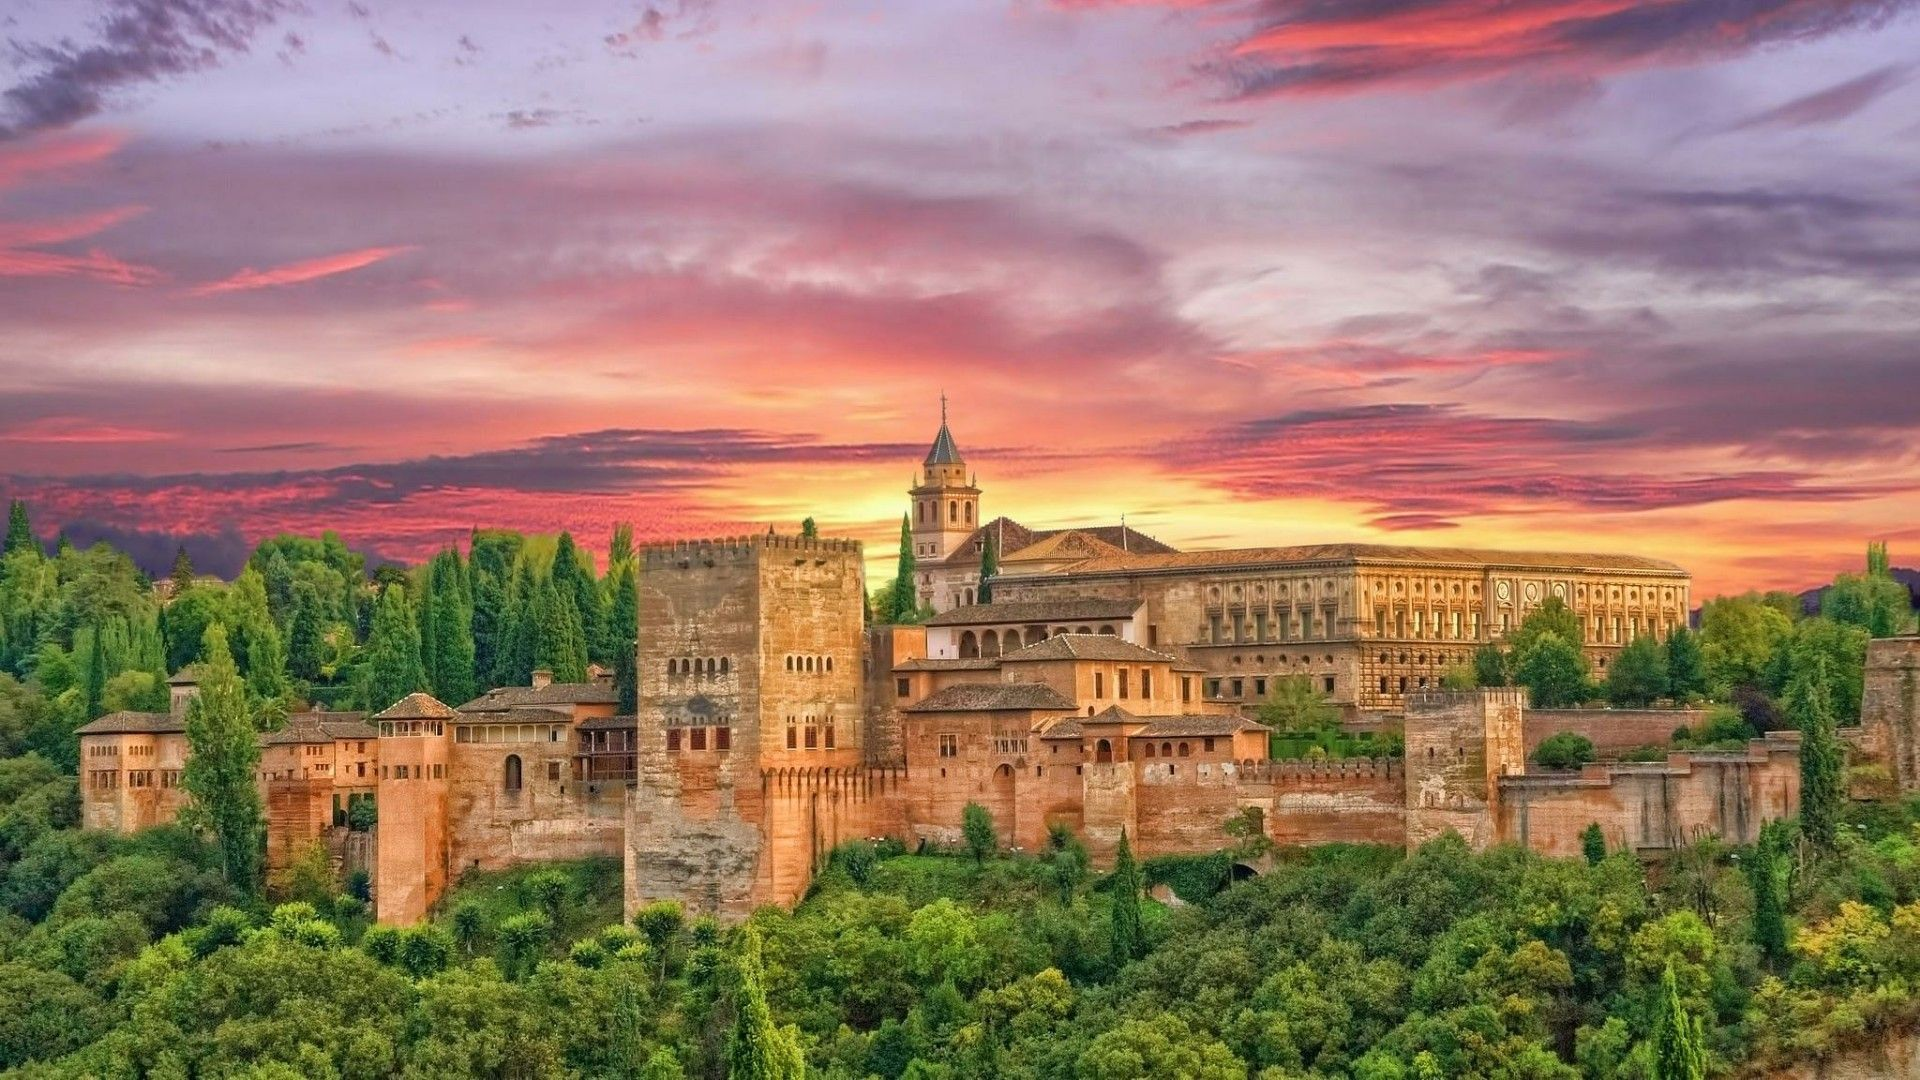
\includegraphics[width=\paperwidth,height=\paperheight,keepaspectratio]{images/granada.jpg}}
}

% Inicio del documento
\begin{document}

% Portada
\maketitle
\thispagestyle{empty}

\begin{center}
    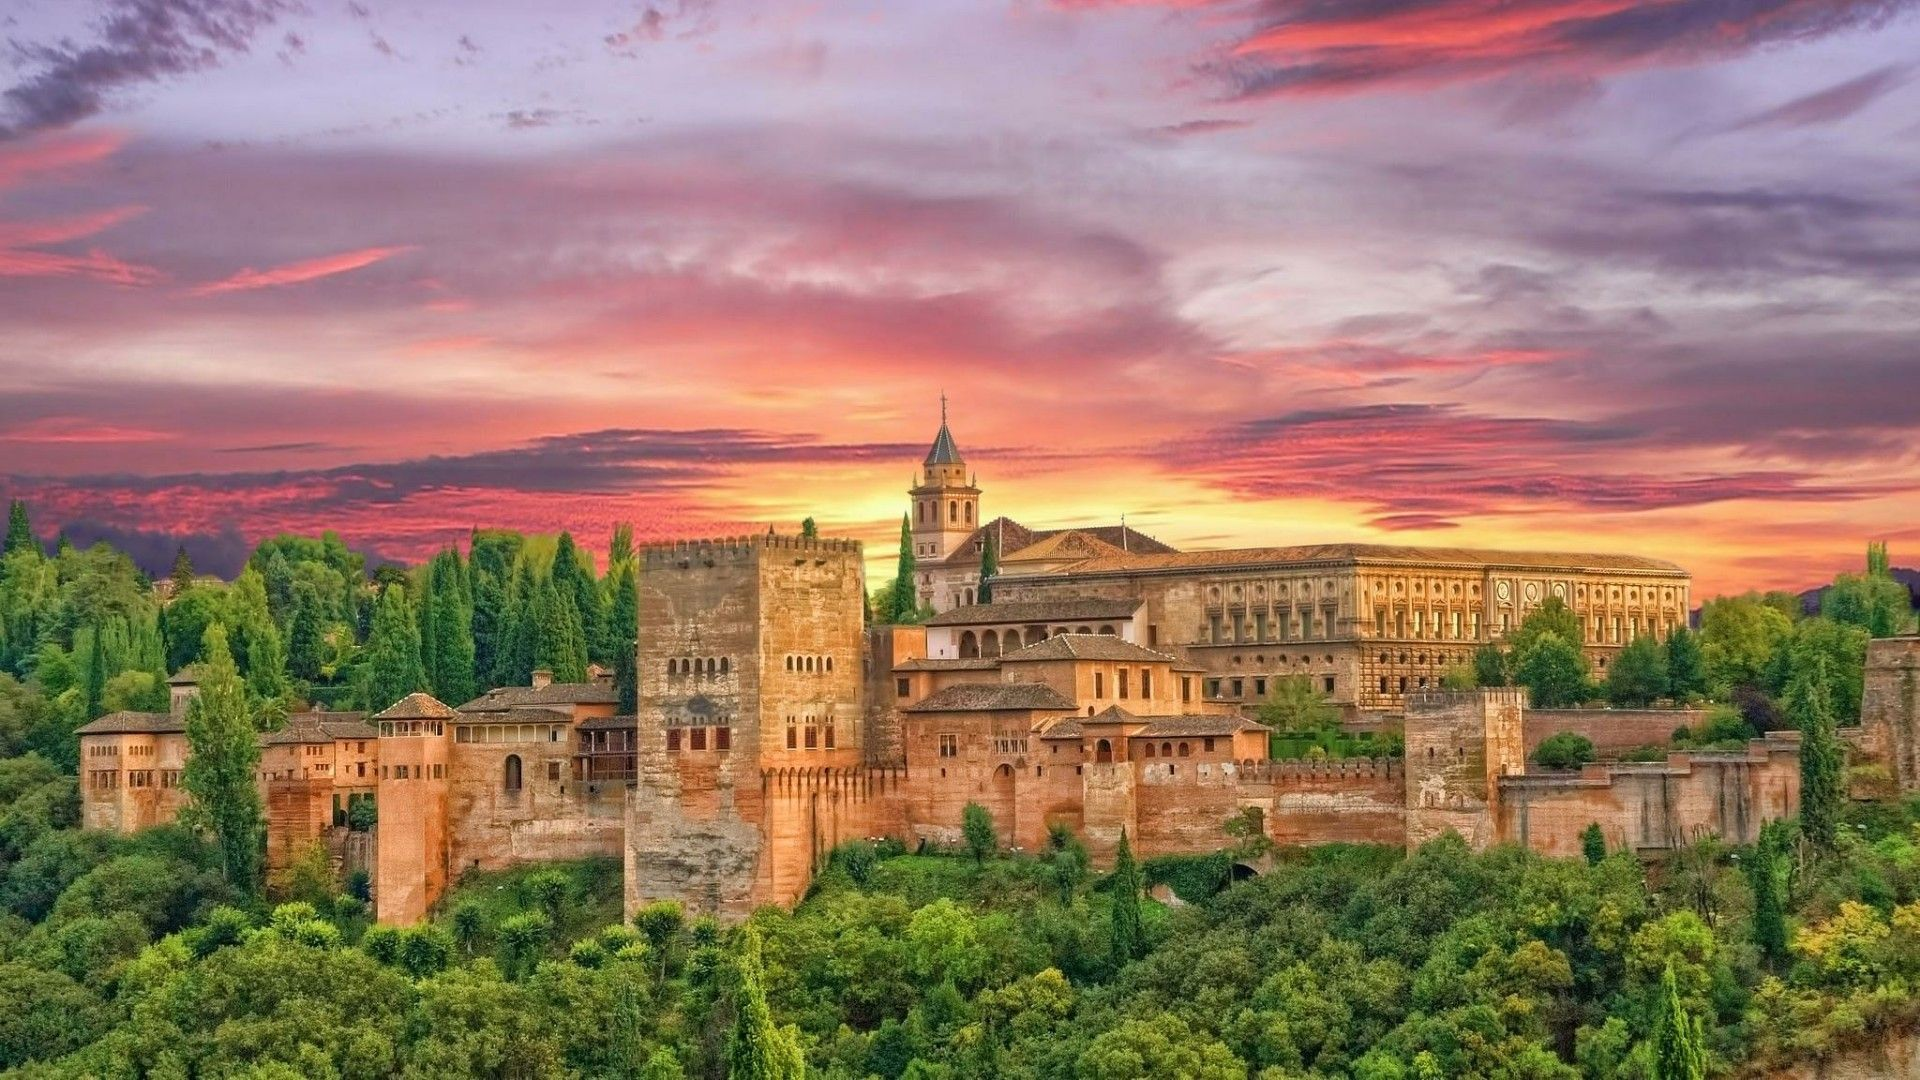
\includegraphics[width=\textwidth,height=0.4\textheight,keepaspectratio]{images/granada.jpg} \\ % Añade tu imagen de fondo
    \vfill
\end{center}

\newpage

% Índice (opcional)
\tableofcontents
\newpage

\section{Ejercicio 91}
\subsection{Enunciado}
Dado el conjunto de tareas periódicas y sus atributos temporales que se indica en la tabla de aquí abajo, determinar si se puede planificar el conjunto de dichas tareas utilizando un esquema de planificación basado en planificación cíclica. Diseña el plan cíclico determinando el marco secundario, y el entrelazamiento de las tareas sobre un cronograma.

\begin{table}[H]
\centering
\begin{tabular}{|c|c|c|c|}
\hline
\textbf{Tarea} & \textbf{Ci} & \textbf{Ti} & \textbf{Di} \\ \hline
T1 & 10 & 40 & 40 \\ \hline
T2 & 18 & 50 & 50 \\ \hline
T3 & 10 & 200 & 200 \\ \hline
T4 & 20 & 200 & 200 \\ \hline
\end{tabular}
\caption{Conjunto de tareas periódicas y sus atributos temporales}
\end{table}

\subsection{Solución}

\begin{tcolorbox}[colback=gray!5!white,colframe=gray!75!black]
    \textit{Nota: El código proporcionado en el enunciado se accede pinchando }\href{https://github.com/ElblogdeIsmael/ElblogdeIsmael.github.io/blob/main/Asignaturas/Tercer%20A%C3%B1o/SCD/Practicas/Practicas_Resueltas/Practica4/scd-p4-fuentes/SOLUCION_ACTIVIDAD_CLASE/ejecutivo2.cpp}{\textit{aquí}}.
\end{tcolorbox}

Para resolver este ejercicio aparte de poseer los conceptos teóricos necesarios de las diapositivas, vamos a servirnos de la metodología de resolución aprendida en prácticas. Este ejercicio al ser el primera será más \textit{didáctico} que el resto.

En base a este tabla:

\begin{table}[H]
    \centering
    \begin{tabular}{|c|c|c|c|}
    \hline
    \textbf{Tarea} & \textbf{Ci} & \textbf{Ti} & \textbf{Di} \\ \hline
    T1 & 10 & 40 & 40 \\ \hline
    T2 & 18 & 50 & 50 \\ \hline
    T3 & 10 & 200 & 200 \\ \hline
    T4 & 20 & 200 & 200 \\ \hline
    \end{tabular}
    \caption{Conjunto de tareas periódicas y sus atributos temporales}
\end{table}

Podemos afirmar que \[D_i = T_i \] (Para hacerlo mas similar al cpp\footnote{Proporcionado en el enlace del inicio de esta sección.}),  por lo que podemos eliminar esa columna y quedarnos con:

\begin{table}[H]
    \centering
    \begin{tabular}{|c|c|c|}
    \hline
    \textbf{Tarea} & \textbf{Ci} & \textbf{Ti} \\ \hline
    T1 & 10 & 40 \\ \hline
    T2 & 18 & 50 \\ \hline
    T3 & 10 & 200 \\ \hline
    T4 & 20 & 200 \\ \hline
    \end{tabular}
    \caption{Conjunto de tareas periódicas y sus atributos temporales}
\end{table}

Tenemos que el ciclo principal dura $T_m = mcm(T_i)\,\forall \, i 0,\ldots, 4 = 200$, de manera que nuestro ciclo secundario debe de cumplir:
\begin{enumerate}
    \item $\max(C_i) \leq T_s \leq \min(D_i)$
    \item $T_s$ divide a $T_m$, siendo el resultado $\in \mathbb{Z}$
\end{enumerate}
Vemos que hay ciertos problemas con el valor 50, ya que según las dos restricciones mencionadas anteriormente, no se puede cumplir ya que si cogemos $T_s = 20ms$ , este no divide a 50, por lo que \textit{no se puede planificar}.

\subsubsection{Cronograma}

\begin{table}[H]
    \centering
    \begin{tabular}{|p{1.4cm}|p{1.2cm}|p{1.2cm}|p{1.2cm}|p{1.2cm}|p{1.2cm}|p{1.2cm}|p{1.2cm}|p{1.2cm}|p{1.2cm}|p{1.2cm}|}
    \hline
    \textbf{Tiempo (ms)} & 0-20 & 20-40 & 40-60 & 60-80 & 80-100 & 100-120 & 120-140 & 140-160 & 160-180 & 180-200 \\ \hline
    \textbf{T1} & X & X & X & X & X & - & - & - & - & - \\ \hline
    \textbf{T2} & - & X & - & X & - & X & - & - & - & - \\ \hline
    \textbf{T3} & - & - & - & - & - & - & X & - & - & X \\ \hline
    \textbf{T4} & - & - & - & - & - & X & - & - & - & X \\ \hline
    \end{tabular}
    \caption{Cronograma de ejecución de las tareas}
\end{table}
    
\subsubsection{Implementación en pseudo-código}


\begin{lstlisting}[style = customcpp, caption = {Implementación en C++ del planificador cíclico}]

    Ts := duración del ciclo secundario;
    ini_sec := instante de inicio del ciclo secundario;

    while (true) { // ciclo principal
        for (desde i := 1 hasta 10) { // 10 porque son las fases del ciclo secundario en base a nuestro cronograma

            inicio_iteracion := instante actual;

            switch(i) {
                case 1:
                case 2:
                case 3:
                case 4:
                case 5:
                    Tarea1();
                    if (i % 2 == 0) { // T2 ejecuta cada 2 marcos
                        Tarea2();
                    }
                    break;

                case 6:
                    Tarea2();
                    Tarea4();
                    break;

                case 7:
                case 9:
                    Tarea3();
                    break;

                case 8:
                    Tarea3();
                    Tarea4();
                    break;

                case 10:
                    Tarea4();
                    break;
            }

            ini_sec += Ts; // siguiente instante
            sleep_until(ini_sec); // esperar hasta el siguiente ciclo secundario
            fin_iteracion := instante actual; // medir retraso
            retraso := fin_iteracion - ini_sec; // calcular retraso
        }
    }
\end{lstlisting}



% \subsection{Solución}

% \begin{tcolorbox}[colback=gray!5!white,colframe=blue!75!black]
%     \textit{En este ejercicio al ser el primero se proporcionarán 3 soluciones válidas, después se continuará con la 2 solución, la que esta basada en la teoría de la Asignatura.}
% \end{tcolorbox}

% Para determinar si el conjunto de tareas puede ser planificado utilizando un esquema de planificación cíclica, procedemos con los siguientes pasos:

% \begin{enumerate}
%     \item \textbf{Cálculo del marco secundario ($S$):}
%     \begin{itemize}
%         \item El marco secundario debe cumplir las siguientes restricciones:
%         \begin{equation}
%         \text{Mínimo común divisor} \leq S \leq \text{Mínimo periodo de las tareas}
%         \end{equation}
%         \begin{equation}
%         \frac{T_i}{S} \in \mathbb{Z}, \quad \forall i
%         \end{equation}
%         \item Aquí, el mínimo común divisor de los periodos es:
%         \[
%         \text{MCD}(40, 50, 200, 200) = 10
%         \]
%         El mínimo periodo es $40$. Por lo tanto, $S$ debe estar en el rango $10 \leq S \leq 40$.
%         \item Probamos divisores en el rango: $S = 10, 20, 40$. Elegimos el valor que satisface todas las condiciones.
%     \end{itemize}

%     \item \textbf{Diseño del plan cíclico:}
%     \begin{itemize}
%         \item Construimos un plan cíclico asignando las tareas a intervalos de tiempo de acuerdo con sus periodos y tiempos de ejecución ($C_i$). 
%         \item Aseguramos que la suma de los tiempos de ejecución de las tareas dentro de un marco no exceda $S$.
%     \end{itemize}

%     \item \textbf{Construcción del cronograma:}
%     \begin{itemize}
%         \item Basándonos en el plan cíclico, construimos un cronograma que muestre el entrelazamiento de las tareas en el tiempo.
%     \end{itemize}
% \end{enumerate}

% \subsubsection{Cálculo del marco secundario}

% El marco secundario $S$ debe cumplir:
% \[
% \text{MCD}(40, 50, 200, 200) = 10, \quad \text{y } S \leq 40.
% \]
% Probamos divisores: $S = 10, 20, 40$. Al probar, encontramos que $S = 20$ satisface todas las condiciones.

% \subsubsection{Diseño del cronograma}

% Con $S = 20$, asignamos las tareas en bloques de tiempo. El diseño del plan cíclico queda como sigue:

% \begin{verbatim}
% Marco 1: T1, T2
% Marco 2: T1
% Marco 3: T3
% Marco 4: T4
% \end{verbatim}

% \subsubsection{Visualización del cronograma}

% El cronograma resultante es:

% \begin{table}[H]
% \centering
% \begin{tabular}{|c|c|c|c|c|}
% \hline
% \textbf{Marco} & \textbf{0--20} & \textbf{20--40} & \textbf{40--60} & \textbf{60--80} \\ \hline
% \textbf{Tareas} & T1, T2 & T1 & T3 & T4 \\ \hline
% \end{tabular}
% \caption{Cronograma del plan cíclico}
% \end{table}

% Por lo tanto, el conjunto de tareas es planificable utilizando un esquema de planificación cíclica.

% \subsection{Solución basada en la teoría}

% De acuerdo con la teoría de planificación cíclica, los pasos para resolver el problema son los siguientes:

% \begin{enumerate}
%     \item \textbf{Cálculo del hiperperiodo ($T_M$):}
%     \begin{itemize}
%         \item El hiperperiodo es el mínimo común múltiplo de los periodos de las tareas ($T_i$):
%         \[
%         T_M = \text{mcm}(40, 50, 200) = 200
%         \]
%         Este valor indica la duración del ciclo principal de planificación.
%     \end{itemize}

%     \item \textbf{Determinación del marco secundario ($T_S$):}
%     \begin{itemize}
%         \item Según la teoría, el marco secundario debe cumplir:
%         \[
%         \text{máximo } C_i \leq T_S \leq \text{mínimo } D_i
%         \]
%         \[
%         T_S \text{ divide exactamente a } T_M
%         \]
%         En este caso:
%         \[
%         \max(C_i) = 20, \quad \min(D_i) = 40
%         \]
%         Probamos divisores de 200 en el rango $20 \leq T_S \leq 40$: los valores posibles son $20$ y $40$. Seleccionamos $T_S = 20$ para optimizar el ajuste.
%     \end{itemize}

%     \item \textbf{Construcción del plan cíclico:}
%     \begin{itemize}
%         \item Dividimos el hiperperiodo en $T_M / T_S = 200 / 20 = 10$ marcos secundarios.
%         \item Asignamos las tareas a cada marco respetando sus periodos y tiempos de ejecución ($C_i$).
%     \end{itemize}
% \end{enumerate}

% \subsubsection{Plan cíclico diseñado}

% El plan cíclico diseñado con $T_S = 20$ se muestra a continuación:

% \begin{table}[H]
% \centering
% \begin{tabular}{|c|c|c|c|c|}
% \hline
% \textbf{Marco} & \textbf{0--20} & \textbf{20--40} & \textbf{40--60} & \textbf{60--80} \\ \hline
% \textbf{Tareas} & T1, T2 & T1 & T3 & T4 \\ \hline
% \end{tabular}
% \caption{Cronograma parcial del plan cíclico}
% \end{table}

% El cronograma completo repite este patrón hasta completar el hiperperiodo de $200$.

% \subsubsection{Validación de la planificabilidad}

% Verificamos que cada tarea cumple su plazo de respuesta:
% \begin{itemize}
%     \item $T1$: Ejecutada cada 40 ms, dentro de su plazo $D_1 = 40$.
%     \item $T2$: Ejecutada cada 50 ms, dentro de su plazo $D_2 = 50$.
%     \item $T3$: Ejecutada cada 200 ms, dentro de su plazo $D_3 = 200$.
%     \item $T4$: Ejecutada cada 200 ms, dentro de su plazo $D_4 = 200$.
% \end{itemize}

% Por lo tanto, el sistema es planificable con el esquema de planificación cíclica.

% \subsubsection{Extra}
% En la tabla, los valores $T_i$, $D_i$, y $C_i$ corresponden a los principales atributos temporales de una tarea en sistemas de tiempo real, según la teoría explicada en tu documento. Estos son:

% \begin{itemize}
%     \item $T_i$: Periodo de la tarea
%     \begin{itemize}
%         \item Es el intervalo de tiempo entre activaciones consecutivas de la tarea.
%         \item Indica cada cuánto tiempo debe ejecutarse la tarea.
%         \item Ejemplo: Para $T_1=40$, la tarea $T_1$ debe activarse cada 40 milisegundos.
%     \end{itemize}

%     \item $D_i$: Deadline o plazo de respuesta máximo
%     \begin{itemize}
%         \item Es el tiempo límite dentro del cual la tarea debe completarse después de ser activada.
%         \item Usualmente, $D_i$ coincide con el periodo $T_i$, pero no necesariamente (puede ser menor).
%         \item Ejemplo: $D_1=40$ significa que $T_1$ debe completarse dentro de 40 milisegundos tras su activación.
%     \end{itemize}

%     \item $C_i$: Tiempo de cómputo máximo
%     \begin{itemize}
%         \item Es el tiempo máximo requerido por la tarea para completar su ejecución, bajo las peores condiciones posibles (WCET, Worst Case Execution Time).
%         \item Este valor representa el recurso temporal mínimo que necesita la tarea en cada activación.
%         \item Ejemplo: $C_1=10$ significa que $T_1$ necesita un máximo de 10 milisegundos de tiempo de procesador para completarse.
%     \end{itemize}
% \end{itemize}

% En resumen:
% \begin{itemize}
%     \item $T_i$: Cada cuánto se activa la tarea.
%     \item $D_i$: Cuándo debe haber terminado como máximo.
%     \item $C_i$: Cuánto tiempo de CPU necesita para completarse.
% \end{itemize}

% \subsection{Solución ajustada al código proporcionado}
% \begin{tcolorbox}[colback=gray!5!white,colframe=gray!75!black]
%     \textit{Nota: El código proporcionado en el enunciado se accede pinchando }\href{https://github.com/ElblogdeIsmael/ElblogdeIsmael.github.io/blob/main/Asignaturas/Tercer%20A%C3%B1o/SCD/Practicas/Practicas_Resueltas/Practica4/scd-p4-fuentes/SOLUCION_ACTIVIDAD_CLASE/ejecutivo2.cpp}{\textit{aquí}}.
% \end{tcolorbox}


% A continuación, presentamos una solución para el problema utilizando los datos del código y basándonos en los principios de planificación cíclica:
% \subsubsection{Código}
% \begin{lstlisting}[style=customcpp, caption={Solución al problema de planificación cíclica}]
% // ------------------------------------------
% // Solución al ejercicio 91 basada en planificación cíclica
% // 
% // Implementación del ejecutivo cíclico:
% // Datos de las tareas:
% // ------------
% // Ta.   T     C
% // ------------
% // T1    40    10
% // T2    50    18
% // T3    200   10
% // T4    200   20
% // ------------
% // 
% // Planificación diseñada con Ts == 20 ms:
% //  *-----------*-----------*-----------*-----------*
% //  | T1 T2     | T1        | T3        | T4        |
% //  *-----------*-----------*-----------*-----------*
% // 
% // ----------------------------------------------------

% #include <string>
% #include <iostream>
% #include <thread>
% #include <chrono>
% #include <iomanip>

% using namespace std;
% using namespace std::chrono;
% using namespace std::this_thread;

% // Tipo para duraciones en segundos y milisegundos, en coma flotante
% typedef duration<float, ratio<1, 1000>> milliseconds_f;

% // Función genérica para representar tareas
% void Tarea(const std::string &nombre, milliseconds tcomputo)
% {
%     cout << "   Comienza tarea " << nombre << " (C == " << tcomputo.count() << " ms.) ... ";
%     sleep_for(tcomputo);
%     cout << "fin." << endl;
% }

% // Tareas específicas del problema
% void Tarea1() { Tarea("T1", milliseconds(10)); }
% void Tarea2() { Tarea("T2", milliseconds(18)); }
% void Tarea3() { Tarea("T3", milliseconds(10)); }
% void Tarea4() { Tarea("T4", milliseconds(20)); }

% int main()
% {
%     // Definición del marco secundario
%     const milliseconds Ts_ms(20);

%     // Instante de inicio del ciclo principal
%     time_point<steady_clock> ini_sec = steady_clock::now();

%     while (true) // Ciclo principal
%     {
%         cout << endl
%              << "---------------------------------------" << endl
%              << "Comienza iteración del ciclo principal." << endl;

%         for (int i = 1; i <= 4; i++) // Ciclo secundario (4 iteraciones)
%         {
%             cout << endl
%                  << "Comienza iteración " << i << " del ciclo secundario." << endl;

%             time_point<steady_clock> inicio_iteracion = steady_clock::now();

%             switch (i)
%             {
%             case 1:
%                 Tarea1();
%                 Tarea2();
%                 break;
%             case 2:
%                 Tarea1();
%                 break;
%             case 3:
%                 Tarea3();
%                 break;
%             case 4:
%                 Tarea4();
%                 break;
%             }

%             // Calcular el siguiente instante de inicio
%             ini_sec += Ts_ms;

%             // Esperar hasta el siguiente ciclo secundario
%             sleep_until(ini_sec);

%             // Medir el retraso respecto al tiempo teórico esperado
%             time_point<steady_clock> fin_iteracion = steady_clock::now();
%             milliseconds_f retraso = milliseconds_f(fin_iteracion - ini_sec);
%             cout << "Retraso al final de la iteración " << i << ": " << retraso.count() << " ms." << endl;
%         }
%     }
% }

% \end{lstlisting}

% \subsubsection{Explicación}

% \paragraph{Cálculo del Marco Secundario $T_S$:}
% \begin{itemize}
%     \item Restricciones de $T_S$:
%         \begin{itemize}
%             \item $\text{máximo } C_i = 20\,\text{ms}$.
%             \item $T_S$ divide a $T_M = \text{mcm}(40, 50, 200) = 200\,\text{ms}$.
%         \end{itemize}
%     \item Elegimos $T_S = 20\,\text{ms}$.
% \end{itemize}

% \paragraph{Planificación de las Tareas:}
% \begin{itemize}
%     \item Ciclo principal con $T_M = 200\,\text{ms}$, dividido en 10 marcos secundarios de $T_S = 20\,\text{ms}$.
%     \item Asignación de las tareas:
%         \begin{itemize}
%             \item Marco 1: $T_1, T_2$
%             \item Marco 2: $T_1$
%             \item Marco 3: $T_3$
%             \item Marco 4: $T_4$
%         \end{itemize}
% \end{itemize}

% \paragraph{Conclusión:}
% \begin{itemize}
%     \item La planificación cíclica es correcta y asegura que todas las tareas cumplen sus plazos ($D_i = T_i$).
%     \item El sistema es planificable usando $T_S = 20\,\text{ms}$.
% \end{itemize}

\section{Ejercicio 92}
\subsection{Enunciado}
El siguiente conjunto de tareas periódicas se puede planificar con ejecutivos cíclicos. Determina si esto es cierto calculando el marco secundario que debería tener. Dibuja el cronograma que muestre las ocurrencias de cada tarea y su entrelazamiento. ¿Cómo se tendría que implementar? (escribe el pseudo-código de la implementación).

\begin{table}[H]
\centering
\begin{tabular}{|c|c|c|c|}
\hline
\textbf{Tarea} & \textbf{Ci} & \textbf{Ti} & \textbf{Di} \\ \hline
T1 & 2 & 6 & 6 \\ \hline
T2 & 2 & 8 & 8 \\ \hline
T3 & 3 & 12 & 12 \\ \hline
\end{tabular}
\caption{Conjunto de tareas periódicas y sus atributos temporales}
\end{table}

\subsection{Solución}
\begin{tcolorbox}[colback=gray!5!white,colframe=gray!75!black]
    \textit{Nota: Este ejercicio se resolverá siguiendo las metodologías vistas en clase y prácticas.}
\end{tcolorbox}

\subsubsection{Paso 1: Verificación inicial}
Podemos observar que \(D_i = T_i\) para todas las tareas, lo que simplifica la verificación inicial. Esto significa que podemos eliminar la columna \(D_i\) y trabajar únicamente con \(C_i\) y \(T_i\):

\begin{table}[H]
\centering
\begin{tabular}{|c|c|c|}
\hline
\textbf{Tarea} & \textbf{Ci} & \textbf{Ti} \\ \hline
T1 & 2 & 6 \\ \hline
T2 & 2 & 8 \\ \hline
T3 & 3 & 12 \\ \hline
\end{tabular}
\caption{Conjunto simplificado de tareas periódicas}
\end{table}

\subsubsection{Paso 2: Cálculo del marco secundario}
El ciclo principal es el mínimo común múltiplo de los períodos \(T_i\):
\[ T_m = \text{mcm}(6, 8, 12) = 24 \text{ ms} \]

El marco secundario \(T_s\) debe cumplir:
\begin{enumerate}
    \item \(\max(C_i) \leq T_s \leq \min(T_i)\)
    \item \(T_s\) divide a \(T_m\) de manera exacta (\(T_m / T_s \in \mathbb{Z}\)).
\end{enumerate}

\textbf{Restricción 1:} \(\max(C_i) = 3 \leq T_s \leq \min(T_i) = 6\).

\textbf{Restricción 2:} \(T_s\) debe dividir a \(T_m = 24\). Los divisores de 24 dentro del rango permitido son:\[T_s = 3, 4, 6\].

Escogemos \(T_s = 6\) ya que cumple con ambas restricciones.

\subsubsection{Paso 3: Cronograma}
Dado \(T_s = 6\), construimos el cronograma:

\begin{table}[H]
\centering
\begin{tabular}{|c|c|c|c|c|c|c|}
\hline
\textbf{Tiempo (ms)} & 0-6 & 6-12 & 12-18 & 18-24 \\ \hline
\textbf{T1} & X & X & X & X \\
\textbf{T2} & - & X & - & X \\
\textbf{T3} & - & - & X & - \\
\hline
\end{tabular}
\caption{Cronograma de ejecución de las tareas}
\end{table}

\subsubsection{Paso 4: Implementación en pseudo-código}

\begin{lstlisting}[style = customcpp, caption = {Implementación en C++ del planificador cíclico}]

    Ts := duración del ciclo secundario;
    ini_sec := instante de inicio del ciclo secundario;
    while(true){ //ciclo principal
        for(desde i hasta 4){ // 4 porque son las fases del ciclo secundario en base a nuestro cronograma

            inicio_iteracion := instante actual;

            switch(i){
                case 1:
                    Tarea1();
                    break;
                case 2:
                    Tarea1();
                    Tarea2();
                    break;
                case 3:
                    Tarea1();
                    Tarea3();
                    break;
                case 4:
                    Tarea1();
                    Tarea2();
                    break;
                
            }

            ini_sec += Ts; //siguiente instante
            sleep_until(ini_sec); //esperar hasta el siguiente ciclo secundario
            fin_iteracion := instante actual; //medir retraso
            retraso := fin_iteracion - ini_sec; //calcular retraso

        }
    }
\end{lstlisting}

Con esto confirmamos que el conjunto de tareas se puede planificar con un esquema de planificación cíclica utilizando \(T_s = 6\).

\section{Ejercicio 93}
\subsection{Enunciado}
Comprobar si el conjunto de procesos periódicos que se muestra en la siguiente tabla es planificable con el algoritmo RMS utilizando el test basado en el factor de utilización del tiempo del procesador. Si el test no se cumple, ¿debemos descartar que el sistema sea planificable?

\begin{table}[H]
\centering
\begin{tabular}{|c|c|c|}
\hline
\textbf{Tarea} & \textbf{Ci} & \textbf{Ti} \\ \hline
T1 & 9 & 30 \\ \hline
T2 & 10 & 40 \\ \hline
T3 & 10 & 50 \\ \hline
\end{tabular}
\caption{Conjunto de procesos periódicos}
\end{table}

\subsection{Solución}
El algoritmo \textbf{Rate Monotonic Scheduling (RMS)} es un esquema de planificación de tiempo real que asigna prioridades de manera estática a tareas periódicas. Las prioridades están inversamente relacionadas con los periodos (\(T_i\)): menor periodo, mayor prioridad. Este método utiliza el factor de utilización del procesador (\(U\)) para determinar si un conjunto de tareas es planificable.

El test de planificabilidad se basa en:
\[
U = \sum_{i=1}^{N} \frac{C_i}{T_i}, \quad U \leq U_0(N) = N \cdot (2^{\frac{1}{N}} - 1)
\]

Para \(N = 3\):
\[
U_0(3) = 3 \cdot (2^{\frac{1}{3}} - 1) \approx 0.779
\]

Cálculo del factor de utilización:
\[
U = \frac{9}{30} + \frac{10}{40} + \frac{10}{50} = 0.3 + 0.25 + 0.2 = 0.75
\]

\textbf{Conclusión:} El sistema es planificable porque \(U = 0.75 \leq U_0(3) = 0.779\).

Si \(U > U_0(N)\), no podemos descartar automáticamente la planificabilidad. Deberíamos construir un cronograma utilizando un diagrama de Gantt para verificar si todas las tareas cumplen sus plazos.

\subsubsection{Implementación en pseudo-código}

\textit{Nota: podemos implementar el algoritmo RMS en C++ de la siguiente manera usando los módulos ya que sería seguir una lógica similar a la de teoría y prácticas de la Asignatura.}

\begin{lstlisting}[style=customcpp, caption={Implementación en C++ del algoritmo RMS}]
    // Prioridades: T1 > T2 > T3 (porque T1 tiene el menor período)
    while (true) {
        tiempo_actual := instante_actual();
        
        if (tiempo_actual % 30 == 0) {
            ejecutar(T1);
        }
        if (tiempo_actual % 40 == 0) {
            ejecutar(T2);
        }
        if (tiempo_actual % 50 == 0) {
            ejecutar(T3);
        }
        
        tiempo_siguiente := tiempo_actual + intervalo_minimo();
        sleep_until(tiempo_siguiente);
    }
\end{lstlisting}

Este código asegura que las tareas se ejecutan según sus prioridades y periodos definidos. Si necesitas el diagrama de Gantt o más detalles, avísame.

\section{Ejercicio 94}
\subsection{Enunciado}
Considérese el siguiente conjunto de tareas compuesto por tres tareas periódicas:

\begin{table}[H]
\centering
\begin{tabular}{|c|c|c|}
\hline
\textbf{Tarea} & \textbf{Ci} & \textbf{Ti} \\ \hline
T1 & 10 & 40 \\ \hline
T2 & 20 & 60 \\ \hline
T3 & 20 & 80 \\ \hline
\end{tabular}
\caption{Conjunto de tareas periódicas}
\end{table}

Comprobar la planificabilidad del conjunto de tareas con el algoritmo RMS utilizando el test basado en el factor de utilización. Calcular el hiperperiodo y construir el correspondiente cronograma.

\subsection{Solución}
\subsubsection{Cálculo del factor de utilización}
El algoritmo \textbf{Rate Monotonic Scheduling (RMS)} establece que las tareas son planificables si su factor de utilización (\(U\)) cumple:
\[
U = \sum_{i=1}^{N} \frac{C_i}{T_i} \quad \text{y} \quad U \leq U_0(N) = N \cdot (2^{\frac{1}{N}} - 1)
\]

Para \(N = 3\):
\[
U_0(3) = 3 \cdot (2^{\frac{1}{3}} - 1) \approx 0.779
\]

Calculamos \(U\):
\[
U = \frac{10}{40} + \frac{20}{60} + \frac{20}{80} = 0.25 + 0.333 + 0.25 = 0.833
\]

\textbf{Conclusión:} \(U = 0.833 > 0.779\), por lo que el conjunto de tareas no pasa el test basado en el factor de utilización. Sin embargo, esto no significa que el sistema no sea planificable. Es necesario construir el cronograma para verificarlo.

\subsubsection{Cálculo del hiperperiodo}
El hiperperiodo (\(T_m\)) es el mínimo común múltiplo (\(\text{mcm}\)) de los períodos de las tareas:
\[
T_m = \text{mcm}(40, 60, 80) = 240 \, \text{ms}
\]

\subsubsection{Cronograma}
El cronograma muestra las instancias de ejecución de las tareas en el intervalo \([0, T_m]\). Construimos una tabla para reflejar esto:

\begin{table}[H]
\centering
\begin{tabular}{|p{1.4cm}|p{1cm}|p{1cm}|p{1cm}|p{1cm}|p{1cm}|p{1cm}|p{1cm}|p{1cm}|p{1cm}|p{1cm}|p{1 cm}|}
\hline
\textbf{Tiempo (ms)} & 0-10 & 10-20 & 20-30 & 30-40 & 40-60 & 60-80 & 80-100 & 100-120 & 120-140 & 140-160 & \ldots \\ \hline
\textbf{T1} & X & - & X & - & X & - & X & - & X & - & \ldots \\ \hline
\textbf{T2} & - & - & - & X & - & X & - & - & - & X & \ldots \\ \hline
\textbf{T3} & - & - & - & - & - & - & X & - & - & - & \ldots \\ \hline
\end{tabular}
\caption{Cronograma de las tareas para \(T_m = 240\) ms}
\end{table}

\subsubsection{Implementación en pseudo-código}
\begin{lstlisting}[style=customcpp, caption={Implementación en C++ del cronograma}]
    while (true) {
        tiempo_actual := instante_actual();

        if (tiempo_actual % 40 == 0) {
            ejecutar(T1);
        }
        if (tiempo_actual % 60 == 0) {
            ejecutar(T2);
        }
        if (tiempo_actual % 80 == 0) {
            ejecutar(T3);
        }

        tiempo_siguiente := tiempo_actual + intervalo_minimo();
        sleep_until(tiempo_siguiente);
    }
\end{lstlisting}

Con este análisis, verificamos que el cronograma asegura que todas las tareas cumplen sus plazos. Aunque no pasa el test de utilización, el sistema es planificable.

\section{Ejercicio 95}
\subsection{Enunciado}
Comprobar la planificabilidad y construir el cronograma de acuerdo al algoritmo de planificación RMS del siguiente conjunto de tareas periódicas:

\begin{table}[H]
\centering
\begin{tabular}{|c|c|c|}
\hline
\textbf{Tarea} & \textbf{Ci} & \textbf{Ti} \\ \hline
T1 & 20 & 60 \\ \hline
T2 & 20 & 80 \\ \hline
T3 & 20 & 120 \\ \hline
\end{tabular}
\caption{Conjunto de tareas periódicas}
\end{table}

\subsection{Solución}
El algoritmo \textbf{Rate Monotonic Scheduling (RMS)} asigna prioridades de manera estática en función del periodo (\(T_i\)): a menor periodo, mayor prioridad. Verificamos la planificabilidad utilizando el test basado en el factor de utilización del procesador.

\subsubsection{Cálculo del Factor de Utilización}
El factor de utilización se calcula como:
\[
U = \sum_{i=1}^N \frac{C_i}{T_i}
\]
Sustituyendo los valores de las tareas:
\[
U = \frac{20}{60} + \frac{20}{80} + \frac{20}{120} = 0.333 + 0.25 + 0.1667 = 0.7497
\]

El límite de utilización máxima (\(U_0(N)\)) para \(N = 3\) tareas es:
\[
U_0(3) = 3 \cdot (2^{\frac{1}{3}} - 1) \approx 0.779
\]

\textbf{Conclusión:} Como \(U = 0.7497 \leq U_0(3) = 0.779\), el conjunto de tareas es planificable según RMS.

\subsubsection{Cálculo del Hiperperiodo}
El hiperperiodo (\(T_m\)) es el \textbf{mínimo común múltiplo (mcm)} de los períodos de las tareas:
\[
T_m = \text{mcm}(60, 80, 120) = 240 \, \text{ms}
\]

\subsubsection{Cronograma}
El cronograma se construye considerando las instancias de activación de cada tarea en el intervalo \([0, T_m]\), donde cada tarea \(T_i\) se activa cada \(T_i\) ms y tiene un tiempo de ejecución de \(C_i\) ms.

\begin{table}[H]
\centering
\begin{tabular}{|c|c|c|c|c|c|c|c|}
\hline
\textbf{Tiempo (ms)} & 0-20 & 20-40 & 40-60 & 60-80 & 80-100 & 100-120 & \ldots \\ \hline
\textbf{T1} & X & - & X & - & X & - & \ldots \\ \hline
\textbf{T2} & - & - & - & X & - & X & \ldots \\ \hline
\textbf{T3} & - & - & - & - & - & - & \ldots \\ \hline
\end{tabular}
\caption{Cronograma de las tareas periódicas para \(T_m = 240\) ms}
\end{table}

\textbf{Nota:} Si se requiere el diagrama de Gantt detallado, puede construirse para el hiperperiodo calculado.

\subsubsection{Implementación en Pseudo-Código}
\begin{lstlisting}[style=customcpp, caption={Implementación en C++ del cronograma}]
    while (true) {
        tiempo_actual := instante_actual();

        if (tiempo_actual % 60 == 0) {
            ejecutar(T1);
        }
        if (tiempo_actual % 80 == 0) {
            ejecutar(T2);
        }
        if (tiempo_actual % 120 == 0) {
            ejecutar(T3);
        }

        tiempo_siguiente := tiempo_actual + intervalo_minimo();
        sleep_until(tiempo_siguiente);
    }
\end{lstlisting}

Con este análisis, concluimos que el conjunto de tareas es planificable y el cronograma asegura el cumplimiento de los plazos.

\section{Ejercicio 96}
\subsection{Enunciado}
Determinar si el siguiente conjunto de tareas puede planificarse con la política de planificación RMS y con la política EDF, utilizando los tests de planificabilidad adecuados para cada uno de los dos casos. Comprobar también la planificabilidad construyendo los cronogramas para ambas políticas.

\begin{table}[H]
\centering
\begin{tabular}{|c|c|c|}
\hline
\textbf{Tarea} & \textbf{Ci} & \textbf{Ti} \\ \hline
T1 & 1 & 5 \\ \hline
T2 & 1 & 10 \\ \hline
T3 & 2 & 20 \\ \hline
T4 & 10 & 20 \\ \hline
T5 & 7 & 100 \\ \hline
\end{tabular}
\caption{Conjunto de tareas periódicas}
\end{table}

\subsection{Solución}
\subsubsection{Planificación con RMS}
El algoritmo \textbf{Rate Monotonic Scheduling (RMS)} asigna prioridades de manera estática en función del periodo (\(T_i\)): a menor periodo, mayor prioridad. Verificamos la planificabilidad utilizando el test basado en el factor de utilización del procesador.

\paragraph{Test de Planificabilidad RMS}
El factor de utilización del procesador se calcula como:
\[
U = \sum_{i=1}^N \frac{C_i}{T_i}
\]

Sustituyendo los valores de las tareas:
\[
U = \frac{1}{5} + \frac{1}{10} + \frac{2}{20} + \frac{10}{20} + \frac{7}{100} = 0.2 + 0.1 + 0.1 + 0.5 + 0.07 = 0.97
\]

El límite de utilización máxima para \(N = 5\) tareas es:
\[
U_0(5) = 5 \cdot (2^{\frac{1}{5}} - 1) \approx 0.743
\]

\textbf{Conclusión:} Como \(U = 0.97 > 0.743\), el sistema \textbf{no pasa el test RMS}. Esto indica que no podemos garantizar la planificabilidad mediante este test.

\paragraph{Construcción del Cronograma RMS}
Para comprobar la planificabilidad con RMS, construimos el cronograma hasta el hiperperiodo (\(T_m\)), que es el \textbf{mcm} de los periodos:
\[
T_m = \text{mcm}(5, 10, 20, 100) = 100 \, \text{ms}
\]

\begin{table}[H]
\centering
\begin{tabular}{|c|c|c|c|c|c|c|}
\hline
\textbf{Tiempo (ms)} & 0-1 & 1-2 & 2-3 & 3-4 & 4-5 & \ldots \\ \hline
\textbf{T1} & X & - & X & - & X & \ldots \\ \hline
\textbf{T2} & - & - & - & - & X & \ldots \\ \hline
\textbf{T3} & - & - & - & X & - & \ldots \\ \hline
\textbf{T4} & - & X & X & X & X & \ldots \\ \hline
\textbf{T5} & - & - & - & - & - & \ldots \\ \hline
\end{tabular}
\caption{Cronograma RMS para \(T_m = 100\) ms}
\end{table}

Si las tareas cumplen sus plazos en \(T_m\), el sistema es planificable con RMS.


\subsubsection{Planificación con EDF}
El algoritmo \textbf{Earliest Deadline First (EDF)} asigna prioridades dinámicamente según los plazos de respuesta (\(d_i\)): a menor plazo restante, mayor prioridad. Este método utiliza el segundo test de planificabilidad de Liu y Layland:
\[
U = \sum_{i=1}^N \frac{C_i}{T_i} \quad \text{y} \quad U \leq 1
\]

\paragraph{Test de Planificabilidad EDF}
Sustituyendo los valores de las tareas:
\[
U = \frac{1}{5} + \frac{1}{10} + \frac{2}{20} + \frac{10}{20} + \frac{7}{100} = 0.97
\]

Dado que \(U = 0.97 \leq 1\), el sistema pasa el test EDF.

\paragraph{Construcción del Cronograma EDF}
Para comprobar la planificabilidad, construimos el cronograma dinámico, priorizando las tareas con menor plazo restante, hasta \(T_m = 100\).

\begin{table}[H]
\centering
\begin{tabular}{|c|c|c|c|c|c|c|}
\hline
\textbf{Tiempo (ms)} & 0-1 & 1-2 & 2-3 & 3-4 & 4-5 & \ldots \\ \hline
\textbf{T1} & X & - & X & - & X & \ldots \\ \hline
\textbf{T2} & - & - & - & - & X & \ldots \\ \hline
\textbf{T4} & - & X & X & X & X & \ldots \\ \hline
\textbf{T3} & - & - & - & X & - & \ldots \\ \hline
\textbf{T5} & - & - & - & - & - & \ldots \\ \hline
\end{tabular}
\caption{Cronograma EDF para \(T_m = 100\) ms}
\end{table}



\subsubsection{Explicación del Algoritmo EDF}
El algoritmo EDF asigna prioridades dinámicas a las tareas en función del tiempo restante hasta su plazo de respuesta absoluto (\(d_i\)). Cuando una tarea se activa, se compara su plazo con el de las demás tareas en cola de ejecución, ejecutándose aquella que tenga el plazo más cercano a expirar. EDF es óptimo para tareas periódicas y aperiódicas si \(U \leq 1\).

Ventajas del EDF:
\begin{itemize}
    \item Mayor utilización del procesador, alcanzando hasta \(U = 1\).
    \item Planificabilidad dinámica para sistemas con alta carga de tareas.
\end{itemize}

\textbf{Nota:} A pesar de pasar el test EDF, el cronograma final debe verificarse para confirmar que todas las tareas cumplen sus plazos.



\section{Ejercicio 97}
\subsection{Enunciado}
Determinar razonadamente si el siguiente conjunto de tareas puede planificarse en un sistema monoprocesador utilizando:
\begin{itemize}
    \item Un \textbf{ejecutivo cíclico}.
    \item Algún algoritmo basado en \textbf{prioridades estáticas} o \textbf{dinámicas}.
\end{itemize}

\begin{table}[H]
\centering
\begin{tabular}{|c|c|c|}
\hline
\textbf{Tarea} & \textbf{Ci} & \textbf{Ti} \\ \hline
T1 & 1 & 5 \\ \hline
T2 & 1 & 10 \\ \hline
T3 & 2 & 10 \\ \hline
T4 & 11 & 20 \\ \hline
T5 & 5 & 100 \\ \hline
\end{tabular}
\caption{Conjunto de tareas periódicas}
\end{table}

\subsection{Solución}
\subsubsection{Planificación mediante un Ejecutivo Cíclico}
El \textbf{ejecutivo cíclico} requiere que las tareas se asignen en ciclos secundarios, garantizando que todas se ejecuten dentro del hiperperiodo. Para que sea planificable:
\[
\text{TM} = \text{mcm}(5, 10, 20, 100) = 100 \, \text{ms}
\]
El tamaño del ciclo secundario (\(TS\)) debe cumplir:
\[
\max(C_i) \leq TS \leq \min(T_i)
\]
En este caso:
\[
\max(C_i) = 11 \quad \text{y} \quad \min(T_i) = 5
\]
Dado que \(11 > 5\), no es posible definir un ciclo secundario que cumpla esta condición. Por lo tanto, el sistema \textbf{no puede planificarse} mediante un ejecutivo cíclico.

\subsubsection{Planificación mediante Prioridades Estáticas (RMS)}
El algoritmo \textbf{Rate Monotonic Scheduling (RMS)} asigna prioridades según los periodos (\(T_i\)): menor \(T_i\), mayor prioridad. Calculamos el factor de utilización del procesador (\(U\)):
\[
U = \sum_{i=1}^N \frac{C_i}{T_i}
\]
Sustituyendo los valores:
\[
U = \frac{1}{5} + \frac{1}{10} + \frac{2}{10} + \frac{11}{20} + \frac{5}{100} = 0.2 + 0.1 + 0.2 + 0.55 + 0.05 = 1.1
\]
El límite de utilización máxima (\(U_0(N)\)) para \(N = 5\) tareas es:
\[
U_0(5) = 5 \cdot (2^{\frac{1}{5}} - 1) \approx 0.743
\]
Dado que \(U = 1.1 > 0.743\), el sistema \textbf{no pasa el test RMS}, y no podemos garantizar su planificabilidad con prioridades estáticas.

\subsubsection{Planificación mediante Prioridades Dinámicas (EDF)}
El algoritmo \textbf{Earliest Deadline First (EDF)} asigna prioridades según los plazos de respuesta (\(d_i\)). El test de planificabilidad EDF verifica si:
\[
U = \sum_{i=1}^N \frac{C_i}{T_i} \leq 1
\]
Sustituyendo los valores:
\[
U = \frac{1}{5} + \frac{1}{10} + \frac{2}{10} + \frac{11}{20} + \frac{5}{100} = 1.1
\]
Dado que \(U = 1.1 > 1\), el sistema \textbf{no pasa el test EDF} y no es planificable con este algoritmo.

\subsubsection{Conclusión}
\begin{itemize}
    \item \textbf{Ejecutivo Cíclico:} No es posible planificar las tareas, ya que no se puede definir un ciclo secundario que cumpla las restricciones de los periodos.
    \item \textbf{Prioridades Estáticas (RMS):} El sistema no pasa el test de utilización RMS, por lo que no es posible garantizar su planificabilidad.
    \item \textbf{Prioridades Dinámicas (EDF):} Aunque EDF es más eficiente, el sistema tampoco pasa el test, ya que el factor de utilización excede \(1\).
\end{itemize}

En resumen, este conjunto de tareas \textbf{no puede planificarse} en un sistema monoprocesador utilizando ninguno de los métodos mencionados.



\section*{Ejercicios Adicionales}


\end{document}